\documentclass[10pt,twocolumn,letterpaper]{article}
\usepackage[pagenumbers]{cvpr}
\usepackage{graphicx}
\usepackage{booktabs}
\usepackage{amsmath}
\usepackage{multirow}
\definecolor{cvprblue}{rgb}{0.21,0.49,0.74}
\usepackage[breaklinks,colorlinks,allcolors=cvprblue]{hyperref}
\graphicspath{{../proposal/figs/pdf/}}

\title{Same Bytes, Different Failures:\\Do Different ViT Compression Routes Fail on the Same Images?}
\author{Manan Kapoor\\
Roll No. 1024030467\\
UCS532 Computer Vision, Sessional Open Challenge, Problem P49}

\begin{document}
\maketitle

\begin{abstract}
P49 asks for a Vision Transformer under 10\,MB. Compression methods are usually compared on clean accuracy at a size computed as \emph{weights $\times$ bits $\div$ 8}. I first show that this formula understates real files by 1.5--53.5\% across five networks, most for small groups and small models. I then compress DeiT-Small four ways (3-bit, ternary, 4-bit with structured pruning, and distillation into DeiT-Tiny with 8-bit storage) to approximately the same \emph{measured} size (9.72--9.80\,MB, within 0.8\%) under an identical 3000-step fine-tuning budget, with three seeds each. Routes of the same size fail on different images: any two routes disagree on 1.2--2.0$\times$ as many images as two seeds of the same route. The clean-image ranking does not survive damage: ternary beats the distilled model on clean images in all seeds ($+0.9$ to $+1.1$ points), and loses on damaged images in all seeds ($-3.7$ to $-3.9$). The uncompressed DeiT-Tiny already explains this reversal. The best model, 3-bit DeiT-Small at 9.718\,MB, loses 3.22 points against the 79.72\% baseline. A smaller file is not a faster model: only the distilled route runs much faster on a CPU (2.2--2.4$\times$), and pruning gains about 10\%. One command rebuilds every number in this report.
\end{abstract}

\section{Introduction}
\label{sec:intro}
A phone or a small camera cannot comfortably hold an 88\,MB model. DeiT-Small~\cite{touvron2021deit} stores 22,050,664 weights in 32 bits; fitting under 10\,MB leaves about 3.6 bits per weight. Three standard tools get there: \emph{quantisation} (store each weight with fewer bits), \emph{structured pruning} (delete whole channels), and \emph{distillation} (train a smaller student to copy a larger teacher).

Comparisons of these tools usually report one number, clean top-1 accuracy, at a size computed on paper. Both hide something. A real file also stores \emph{scales}, which turn rounded codes back into weights, and keeps some layers at 16 bits. And two models with the same accuracy can fail on different images and react differently to noise or blur~\cite{hooker2019forget}.

This project fixes the two things a deployment pays for, measured bytes and training effort, and changes only the compression method. It asks whether routes of approximately the same size fail on the same images, and whether the model that wins on clean images still wins on damaged ones. Contributions:
\begin{itemize}\setlength\itemsep{0pt}
\item A measured audit of real file size against the formula for five networks (\cref{sec:size}).
\item Four routes matched to within 0.8\% in measured size under equal fine-tuning, with a seed floor that separates route effects from seed noise (\cref{sec:method,sec:fail}).
\item Evidence that the clean ranking reverses under damage, traced to the network rather than to distillation (\cref{sec:flip}).
\item The P49 Pareto table of accuracy, size and CPU latency, and a repository where one command rebuilds every table.
\end{itemize}

\section{Related Work}
\label{sec:related}
\textbf{Size accounting.} Language-model quantisation counts scale storage in bits per weight, \eg SpQR~\cite{dettmers2023spqr}. Vision mixed-precision work (Mix-QViT~\cite{ranjan2025mixqvit}, LampQ~\cite{kim2026lampq}) budgets average bits per weight; with one scale per channel this is a fair shortcut (\cref{sec:size}). FTerViT~\cite{rucinski2026ftervit} reports a measured flash footprint (5.81\,MB, 77.47\% for ternary DeiT-Small) after 260 epochs with 8-bit activations, a different regime from this study.

\textbf{Comparing compression methods.} Kuzmin \etal~\cite{kuzmin2023pruning} compare pruning and quantisation under equal fine-tuning at a theoretical size, with unstructured pruning, and test combining them only briefly. I borrow their equal-effort control.

\textbf{What compression breaks.} Hooker \etal~\cite{hooker2019forget} show compression concentrates errors on particular images and amplifies sensitivity to ImageNet-C~\cite{hendrycks2019benchmarking}, comparing compressed with uncompressed models. Miller \etal~\cite{miller2021line} show that accuracy under shift usually follows a linear trend in clean accuracy on probit axes, with noise among the exceptions. Guo \etal~\cite{guo2017calibration} introduce temperature scaling. Ternary weights follow TWN~\cite{li2016ternary}; TinyViT~\cite{wu2022tinyvit} is the distillation reference named in P49.

\section{The Size Formula Versus the Real File}
\label{sec:size}
Every model is written to a raw binary file and measured with \texttt{os.path.getsize()}. For $N$ weights at $b$ bits:
\begin{equation}
S_{\text{real}} = \tfrac{N_q b}{8} + \tfrac{2 N_q}{g} + 2N_k + \text{header},
\label{eq:size}
\end{equation}
where $N_q$ weights are rounded, $g$ weights share each 2-byte scale, and $N_k$ weights (patch embedding, head, norms, biases) stay at 16 bits. The formula keeps only $N b/8$. For all 80 audited files, the measured size equals \cref{eq:size} predicted from layer shapes plus the header (at most 14.6\,KB).

\begin{figure}[t]
\centering
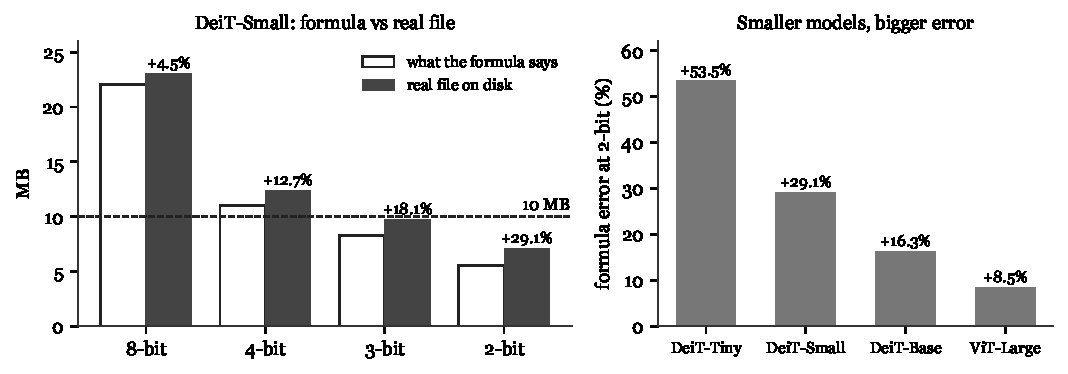
\includegraphics[width=\linewidth]{fig1_size_gap}
\caption{Formula against real file. Left: DeiT-Small, group 256. Right: the 2-bit gap shrinks as networks grow, because the 16-bit layers are a larger share of small networks.}
\label{fig:size}
\end{figure}

For DeiT-Small at group 256 the real file exceeds the formula by 4.5\% at 8 bits, 12.7\% at 4, 18.1\% at 3 and 29.1\% at 2 bits (\cref{fig:size}). At 2 bits the gap is 53.5\% for DeiT-Tiny, 24.5\% for Swin-Tiny, 16.3\% for DeiT-Base and 8.5\% for ViT-Large. A real 4-bit DeiT-Small file is 12.42\,MB, 24\% over the limit, so a 4-bit route must also prune. Mix-QViT's printed 11.4\,MB for 4-bit DeiT-Small rebuilds from the formula; built their way (one scale per channel) a real file is only 2.2--5.4\% larger. The formula is fair for per-channel scales and fails under the small groups a hard 10\,MB budget forces.

\section{Method}
\label{sec:method}
\textbf{Routes.} A \emph{route} is one recipe: compress, then fine-tune. Each has one setting, found by binary search on the written file until it lands just under the target; accuracy is never used. \Cref{tab:main} lists the result.
\begin{itemize}\setlength\itemsep{0pt}
\item \textbf{A, 3-bit}: symmetric group-wise rounding, 36 weights per scale.
\item \textbf{B, ternary}: weights in $\{-1,0,+1\}$ with one scale per row (TWN threshold $0.7\,\mathbb{E}|w|$), five weights per byte ($3^5=243\le256$); the 15 most sensitive layers (by weight variance) stay at 8 bits.
\item \textbf{C, 4-bit + structured pruning}: the 374 weakest of 1,536 MLP channels per block removed (24.3\%), then 4-bit.
\item \textbf{D, distillation}: DeiT-Tiny distilled from DeiT-Small (temperature 2, equal weight with the label loss), stored at 8 bits with 38 layers kept at 16 bits.
\end{itemize}

\textbf{Fine-tuning (identical for all routes).} 3000 steps, batch 256, AdamW, learning rate $10^{-4}$ with cosine decay, weight decay 0.05, label smoothing 0.1, on 200 of 1,024 ImageNet training shards ($\approx$20\%). Rounding is simulated in the forward pass with a straight-through estimator, so full-precision weights keep learning. The exported model is always the step-3000 model; validation accuracy is only logged. Three seeds per route.

\textbf{Evaluation.} Clean top-1 on all 50,000 ImageNet validation images; 14 of the 15 ImageNet-C corruptions~\cite{hendrycks2019benchmarking} at severity 3 on the first 5,000 images (glass blur excluded: 865\,s per 1,000 images, about 20$\times$ the others). Every model saw identical images and damage, and every right/wrong answer is stored per image.

\textbf{Statistics.} Disagreement between models $x,y$ is the share of images where exactly one is right, $d(x,y)=\frac1n\sum_i \mathbb{1}[c_x(i)\neq c_y(i)]$. The \emph{seed floor} is $d$ between two seeds of one route. Paired comparisons use McNemar's exact test and image bootstrap (10,000 resamples) with Bonferroni correction; the 5,000 damaged images, not 70,000 image-corruption pairs, are the unit. Seeds give means, ranges and sign agreement only. Four predictions were written into the analysis script before it ran (\cref{sec:limits}).

\textbf{Checks.} All 21 model files decode and re-encode byte-identically. Every model was re-scored from its file on a different GPU (Kaggle T4, float16); 99.71\% of 600,000 per-image answers match the original run (bfloat16, H100).

\section{Results}
\label{sec:results}
\begin{table*}[t]
\centering
\small
\begin{tabular}{llcccccc}
\toprule
 & Model & File (MB) & Clean top-1 & 3-seed range & Loss & Damaged (14) & CPU ms, Intel / M2 \\
\midrule
 & DeiT-Small, 32-bit & 88.24 & 79.72 & -- & -- & 62.64 & 71.4 / 17.8 \\
A & 3-bit, group 36 & 9.718 & 76.50 & 76.44--76.56 & 3.22 & 55.04 & 71.4 / 17.8 \\
B & ternary & 9.785 & 72.43 & 72.26--72.56 & 7.29 & 44.35 & 71.4 / 17.8 \\
C & 4-bit + pruning & 9.796 & 75.70 & 75.66--75.73 & 4.02 & 53.55 & 64.1 / 16.1 \\
D & DeiT-Tiny, distilled, 8-bit & 9.765 & 71.41 & 71.24--71.54 & 8.31 & 48.16 & 29.9 / 8.0 \\
\bottomrule
\end{tabular}
\caption{Main results (accuracy: mean of 3 seeds, re-scored from the model files). Damaged: mean over 14 corruptions at severity 3 on 5,000 images. CPU: 32-bit kernels, 4 threads, batch 1, median of 50 runs. The published DeiT-Small accuracy is 79.8\%.}
\label{tab:main}
\end{table*}

\subsection{Routes of the same size fail on different images}
\label{sec:fail}
Two seeds of one route disagree on 8.49\% (A), 9.55\% (B), 7.72\% (C) and 6.31\% (D) of the 50,000 clean images. Different routes disagree more in every pair (\cref{fig:seeds}): A--C 9.92\% against a floor of 8.11\% (1.2$\times$), A--B 1.4$\times$, B--C 1.4$\times$, B--D 1.8$\times$, A--D 1.9$\times$, C--D 2.0$\times$. Every 95\% interval of the excess over the floor excludes zero, and on damaged images the ratios are 1.2--1.9$\times$. Routes A and C, both plain quantisation of DeiT-Small, are the most alike.

\begin{figure}[t]
\centering
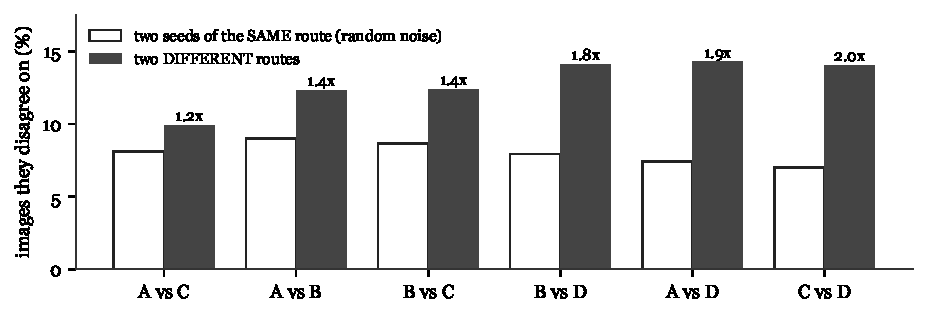
\includegraphics[width=\linewidth]{fig5_routes_vs_seeds}
\caption{Disagreement between two seeds of one route (white) and between two routes (dark), clean images. The ratio is printed on each bar.}
\label{fig:seeds}
\end{figure}

Within DeiT-Small, ternary's deficit grows under damage. Against 3-bit it is 3.46--3.92 points on clean images and 10.35--11.05 on damaged ones; the difference-in-differences is $+6.6$ to $+7.4$ points with every interval excluding zero. By family the deficit is largest for noise (17.7--20.2 points) and smallest for digital damage (5.9--6.4 points).

\subsection{The clean ranking reverses under damage}
\label{sec:flip}
On clean images ternary beats the distilled model in every seed ($+1.02$, $+0.92$, $+1.12$ points; McNemar $p=1.2\times10^{-9}$, $3.3\times10^{-8}$, $1.4\times10^{-11}$). On damaged images the distilled model wins in every seed ($+3.83$, $+3.88$, $+3.71$ points; 95\% intervals $[3.34,4.33]$, $[3.40,4.38]$, $[3.22,4.20]$). All six tests pass the Bonferroni bar $p<0.0083$. On the original corruption set, D is ahead on 11 of 14 corruptions in all three seeds and significantly ahead on 7 (Bonferroni over 14); B is ahead only on elastic, pixelate and JPEG (\cref{fig:rank}).

\begin{figure}[t]
\centering
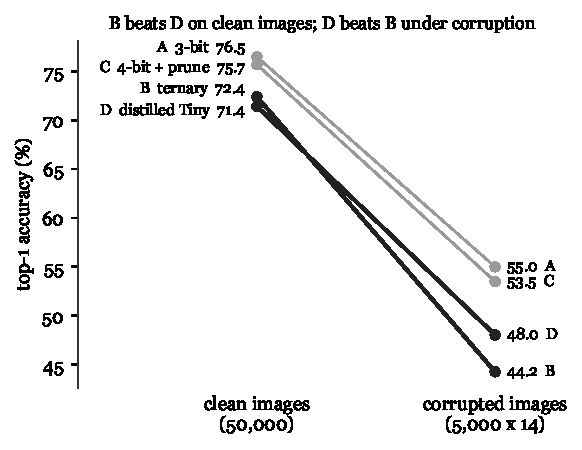
\includegraphics[width=0.78\linewidth]{fig3_two_rankings}\\[2pt]
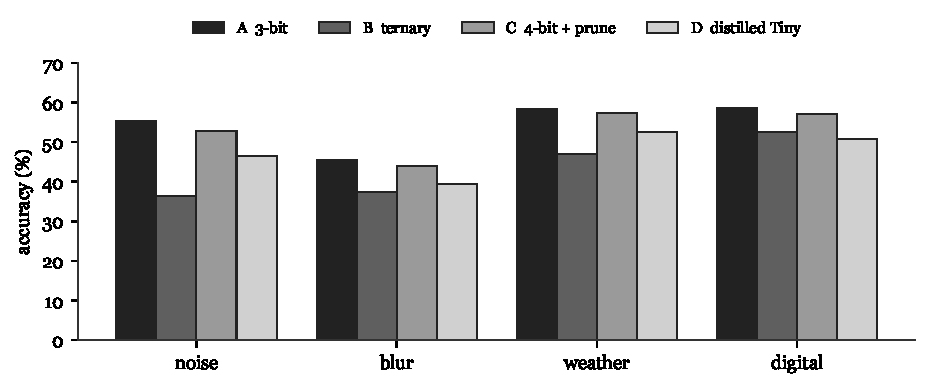
\includegraphics[width=\linewidth]{fig4_families}
\caption{Top: rankings on clean and damaged images; B and D cross. Bottom: accuracy by damage family (mean of 3 seeds).}
\label{fig:rank}
\end{figure}

\textbf{Where D's robustness comes from.} The uncompressed DeiT-Tiny already beats ternary by $+5.51$ points on damaged images; route D beats it by $+3.81$. Distillation and 8-bit storage \emph{lowered} DeiT-Tiny's damaged accuracy by 1.70 points (clean: $-0.61$). The reversal is therefore a property of the smaller network, not of distillation. Since route D also changes the architecture, I report it as a deployment result: choosing on clean accuracy alone picks ternary, which is the wrong model for noisy inputs.

\subsection{Calibration and the trend line}
\label{sec:calib}
Fitting one temperature on the even-numbered images and measuring ECE (15 bins) on the odd ones (\cref{fig:calib}, left), route D goes from the worst calibration (11.84--12.05\%) to the best (2.92--3.14\%); A, B and C end at 3.74--4.32\%. D's miscalibration is a uniform offset, consistent with soft-label distillation.

To ask whether ternary is specially weak on noise or simply weaker (\cref{fig:calib}, right), I fit the clean-to-noise trend of seven same-shape models (route A at five group sizes, plus A and C) on probit axes~\cite{miller2021line}. Ternary sits 4.40--5.03 points below the line in every seed, and the pre-registered 95\% interval excludes zero in all three. It does not survive a Bonferroni-strict 98.3\% interval (2 of 3 seeds include zero) or a plain-axis fit, and ternary's clean accuracy lies about 2 points outside the fitted range. I report it as consistent, not established.

\begin{figure}[t]
\centering
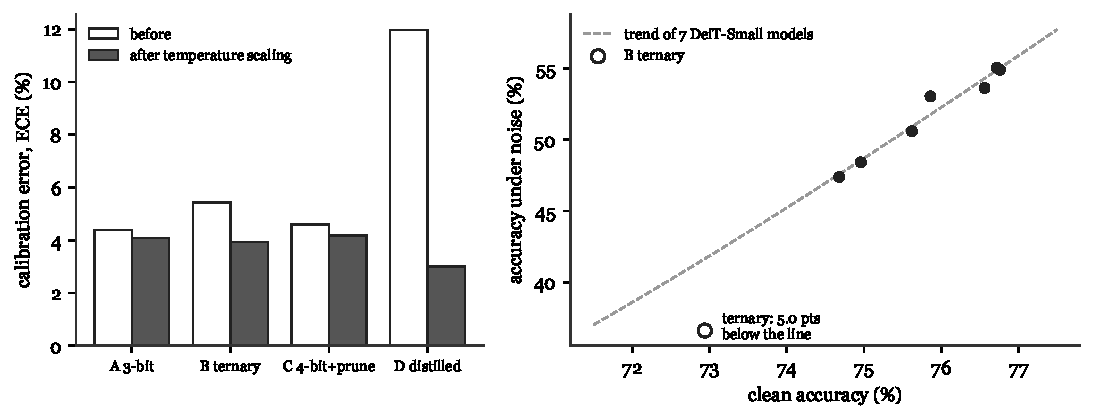
\includegraphics[width=\linewidth]{fig8_calibration_trend}
\caption{Left: ECE before and after temperature scaling (mean of 3 seeds, odd-numbered images). Right: noise accuracy against clean accuracy for seven same-shape models (seed 0), with ternary below the fitted trend.}
\label{fig:calib}
\end{figure}

\subsection{Pareto table: a smaller file is not a faster model}
\label{sec:latency}
Routes A and B are nine times smaller than the original but run at its speed (\cref{tab:main}): no CPU kernel executes 3-bit or ternary weights, so they are expanded at load time. Pruning (C) gains about 10\% (1.11$\times$ on both machines); only the distilled DeiT-Tiny is much faster, 2.23$\times$ on an Apple M2 and 2.38$\times$ on an Intel Xeon (32-bit, 4 threads). A, C and D are Pareto-optimal; B is dominated by A (same speed, 4.1 points lower). PyTorch's dynamic 8-bit quantisation is 4.6--5.7$\times$ slower than 32-bit on the M2 but 1.21$\times$ faster on Intel, so CPU conclusions are machine-specific.

\textbf{What each stage buys.} Rebuilding route A at groups 512 to 36 raises the file from 8.59 to 9.72\,MB and clean accuracy from 74.51 to 76.51\% (damaged 50.07 to 54.90\%). For route D, swapping to DeiT-Tiny costs 7.7 points; distillation and 8-bit to 9.77\,MB cost a further 0.8 (seed 0). Intermediate stages of B and C were not saved.

\section{Limitations and Withdrawn Claims}
\label{sec:limits}
\textbf{Limitations.} Only weights are compressed; activations stay 16-bit, so these accuracies are not comparable with W3A3 papers. Rounding is round-to-nearest, shared by all routes, not GPTQ-style. Fine-tuning used 20\% of ImageNet for 3000 steps and ternary was still improving fastest (0.9--1.4 points over the last 1,000 steps against at most 0.6 for the others), so the ranking belongs to this budget. Sizes span 0.80\%, not an exact match. Sensitivity ranking uses weight variance, a crude proxy. No single model combines all three methods. ImageNet-C is regenerated, so absolute scores differ from published ones. I use ImageNet-1k rather than ImageNet-100, and prune MLP channels rather than tokens (which change the file by zero bytes) or heads.

\textbf{Predictions and withdrawn claims.} Before the analysis I predicted (1) a seed floor of 3--6\% (wrong: 6.3--9.6\%), (2) D beating B on at least 8 of 14 corruptions (held: 11), (3) ternary's gap growing under damage within DeiT-Small (held), and (4) ECE equal to the accuracy--confidence gap (held on clean images only). Three earlier claims were withdrawn after checking: that the size formula misstates published ViT sizes in general (it is fair for per-channel scales); that the ternary noise deficit is established (it fails the strict test); and a comparison of Mix-QViT's size with my group-wise files, which mixed their missing bytes with my different design. Ten pipeline bugs are recorded in the repository; two were visible only because file size was measured alongside accuracy.

\section{Conclusion}
Under a hard size limit, measured bytes, not bits per weight, are the right budget. At approximately equal measured size and equal effort, compression routes are not interchangeable: they fail on different images, beyond seed noise, and the clean ranking can reverse under damage. A deployment choice made on clean accuracy and on paper size can pick a larger, slower or less robust model than intended.

\textbf{Reproducibility.} \texttt{reproduce.sh} rebuilds every statistic and table from the saved per-image results and model files on a laptop in about 90 seconds; six notebooks print the real source of every step.

\textbf{AI-assistance declaration.} AI assistants (Claude, via Claude Code) were used for: writing and debugging the analysis, evaluation and figure code; drafting and editing the proposal and this report; and checking numbers against the evidence and literature claims against the primary papers. All AI-generated code was reviewed, run and checked against the archived outputs with \texttt{reproduce.sh}, and is understood by the author. The following components contain no AI-generated content: \textbf{[to be completed by the author]}.

{\small
\bibliographystyle{ieeenat_fullname}
\bibliography{refs}
}
\end{document}
